%%%%%%%%%%%%%%%%%%%%%%%%%%%%%%%%%%%%%%%%%%%%%%%%%%%%%%%%%%%%%%%%%%%%
%% Presentation: Diabetic Retinopathy Detection - REALISTIC VERSION
%% Phản ánh đúng mô hình thực tế đang implement
%%%%%%%%%%%%%%%%%%%%%%%%%%%%%%%%%%%%%%%%%%%%%%%%%%%%%%%%%%%%%%%%%%%%

\documentclass{beamer}
\usetheme[faculty=wi]{fibeamer}
\usepackage[utf8]{inputenc}
\usepackage[
  main=vietnamese,
  vietnamese
]{babel}

\title{Phát hiện và Phân đoạn Bệnh Võng mạc Tiểu đường sử dụng Deep Learning}
\subtitle{DenseNet + Attention + GRU được tối ưu bằng SANGO}
\date{\today}

\usepackage{ragged2e}
\usepackage{booktabs}
\usepackage{tabularx}
\usepackage{tikz}
\usetikzlibrary{calc, shapes, backgrounds, positioning}
\usepackage{amsmath, amssymb}
\usepackage{url}
\usepackage{graphicx}
\graphicspath{{../outputs/preprocess/}{../outputs/results/gradcam_visualizations/}}
\setbeamersize{text margin left=7mm,text margin right=7mm}
\renewcommand{\arraystretch}{1.15}

\begin{document}

  \begin{darkframes}
    \frame[c]{\maketitle}
  \end{darkframes}

  \AtBeginSection[]{
    \begin{frame}<beamer>
      \frametitle{Nội dung}
      \tableofcontents[currentsection]
    \end{frame}
  }

  \begin{darkframes}

    %% SECTION 1: BÀI TOÁN
    \section{Bài toán}

    \begin{frame}{Giới thiệu bài toán}
      \framesubtitle{Bệnh võng mạc tiểu đường (Diabetic Retinopathy - DR)}

      \begin{block}{Bối cảnh}
        \begin{itemize}
          \item 537 triệu người mắc tiểu đường toàn cầu (2021)
          \item DR là nguyên nhân gây mù lòa ở bệnh nhân tiểu đường
          \item Cần phát hiện sớm để ngăn ngừa mất thị lực
        \end{itemize}
      \end{block}

      \begin{alertblock}{Thách thức}
        \begin{itemize}
          \item \textbf{Dataset nhỏ:} IDRiD chỉ 81 ảnh (54 train, 27 test)
          \item \textbf{Class imbalance:} Phân bố không đều giữa các cấp độ
          \item \textbf{Tổn thương nhỏ:} Microaneurysms chỉ vài pixels
          \item Chất lượng ảnh thấp: độ tương phản thấp, nhiễu
        \end{itemize}
      \end{alertblock}
    \end{frame}

    \begin{frame}{Phân loại bệnh võng mạc tiểu đường}
      \framesubtitle{5 cấp độ nghiêm trọng}

      \begin{columns}[T]
        \column{0.5\textwidth}
        \textbf{Phân loại:}
        \begin{itemize}
          \item Grade 0: No DR
          \item Grade 1: Mild NPDR
          \item Grade 2: Moderate NPDR
          \item Grade 3: Severe NPDR
          \item Grade 4: Proliferative DR (PDR)
        \end{itemize}

        \column{0.5\textwidth}
        \textbf{Tổn thương cần phân đoạn:}
        \begin{itemize}
          \item \alert{Microaneurysms (MA)}
          \item \alert{Hemorrhages (HE)}
          \item \alert{Hard Exudates (EX)}
        \end{itemize}
      \end{columns}

      \vspace{0.5cm}
      \begin{alertblock}{Thách thức segmentation}
        Tổn thương rất nhỏ (< 1\% diện tích ảnh), class imbalance 99:1
      \end{alertblock}
    \end{frame}

    \begin{frame}{Mục tiêu nghiên cứu}
      \begin{enumerate}
        \item \textbf{Tiền xử lý nâng cao:}
        \begin{itemize}
          \item Adaptive Gabor Filter với Chaotic Map
          \item CLAHE (Contrast Limited AHE)
          \item Cải thiện visibility của tổn thương nhỏ
        \end{itemize}

        \item \textbf{Phân đoạn chính xác:}
        \begin{itemize}
          \item Modified U-Net với Adaptive Batch Normalization
          \item Combined Loss (Focal + Tversky + Dice)
          \item Xử lý class imbalance nghiêm trọng
        \end{itemize}

        \item \textbf{Phân loại đa mô hình:}
        \begin{itemize}
          \item DenseNet121 backbone (pretrained ImageNet)
          \item Attention mechanism
          \item Bidirectional GRU với SANGO optimization
        \end{itemize}
      \end{enumerate}
    \end{frame}

    %% SECTION 2: PHƯƠNG PHÁP
    \section{Phương pháp}

    \begin{frame}{Kiến trúc tổng thể}
      \framesubtitle{Two-phase approach}

      \begin{center}
        \begin{tikzpicture}[
          node distance=1.2cm,
          box/.style={rectangle, draw, fill=blue!20, text width=2.2cm, align=center, minimum height=0.8cm, font=\small},
          arrow/.style={->, >=stealth, thick}
        ]
          \node[box] (input) {Ảnh đầu vào\\4288×2848};
          \node[box, right=of input] (preprocess) {Tiền xử lý\\AGF+CLAHE};
          \node[box, below=0.8cm of preprocess] (segment) {Phân đoạn\\U-Net};
          \node[box, left=of segment] (classify) {Phân loại\\DenseNet+GRU};
          \node[box, left=of classify] (output) {Kết quả\\Grade + Mask};

          \draw[arrow] (input) -- (preprocess);
          \draw[arrow] (preprocess) -- (segment);
          \draw[arrow] (preprocess) -- (classify);
          \draw[arrow] (segment) -- (output);
          \draw[arrow] (classify) -- (output);
        \end{tikzpicture}
      \end{center}

      \vspace{0.3cm}
      \begin{block}{Đặc điểm}
        \begin{itemize}
          \item Training riêng biệt: Phase 1 (Classification) → Phase 2 (Segmentation)
          \item Giải thích kết quả: Grad-CAM visualization
        \end{itemize}
      \end{block}
    \end{frame}

    \begin{frame}{Tiền xử lý — Adaptive Gabor Filter}
      \framesubtitle{Kết hợp Chaotic Map}

      \textbf{Chebyshev Chaotic Map:}
      \begin{equation*}
        x_{t+1} = \cos(n \cdot \arccos(x_t))
      \end{equation*}

      \textbf{Adaptive Gabor Kernel:}
      \begin{equation*}
        g(x,y;\theta,\lambda,\sigma,\gamma) =
        \exp\!\left(-\frac{x'^2+\gamma^2 y'^2}{2\sigma^2}\right)
        \cos\!\left(\frac{2\pi x'}{\lambda}+\psi\right)
      \end{equation*}
      với $\theta' = \theta + x_t \cdot 0.1$ (chaotic perturbation)

      \vspace{0.3cm}
      \textbf{Tham số thực tế:}
      \begin{itemize}
        \item Kernel size: 31×31
        \item $\sigma = 3.0$, $\lambda = 10.0$, $\gamma = 0.5$
        \item 8 orientations: $\theta_i = \pi \cdot i / 8$
      \end{itemize}
    \end{frame}

    \begin{frame}{Tiền xử lý — CLAHE}
      \framesubtitle{Contrast Limited Adaptive Histogram Equalization}

      \textbf{Tham số:}
      \begin{itemize}
        \item Clip limit: 2.0
        \item Tile grid: 8×8
        \item Áp dụng trên LAB color space (L channel)
      \end{itemize}

      \vspace{0.5cm}
      \textbf{Công thức:}
      \[
        \beta = \frac{M}{N}\left(1+\frac{\alpha}{100}S_{\max}\right)
      \]
      \[
        gr_{out} = (gr_{\max}-gr_{\min}) \cdot CDF(gr_{in}) + gr_{\min}
      \]
    \end{frame}

    \begin{frame}{Tiền xử lý — Kết quả}
      \begin{center}
        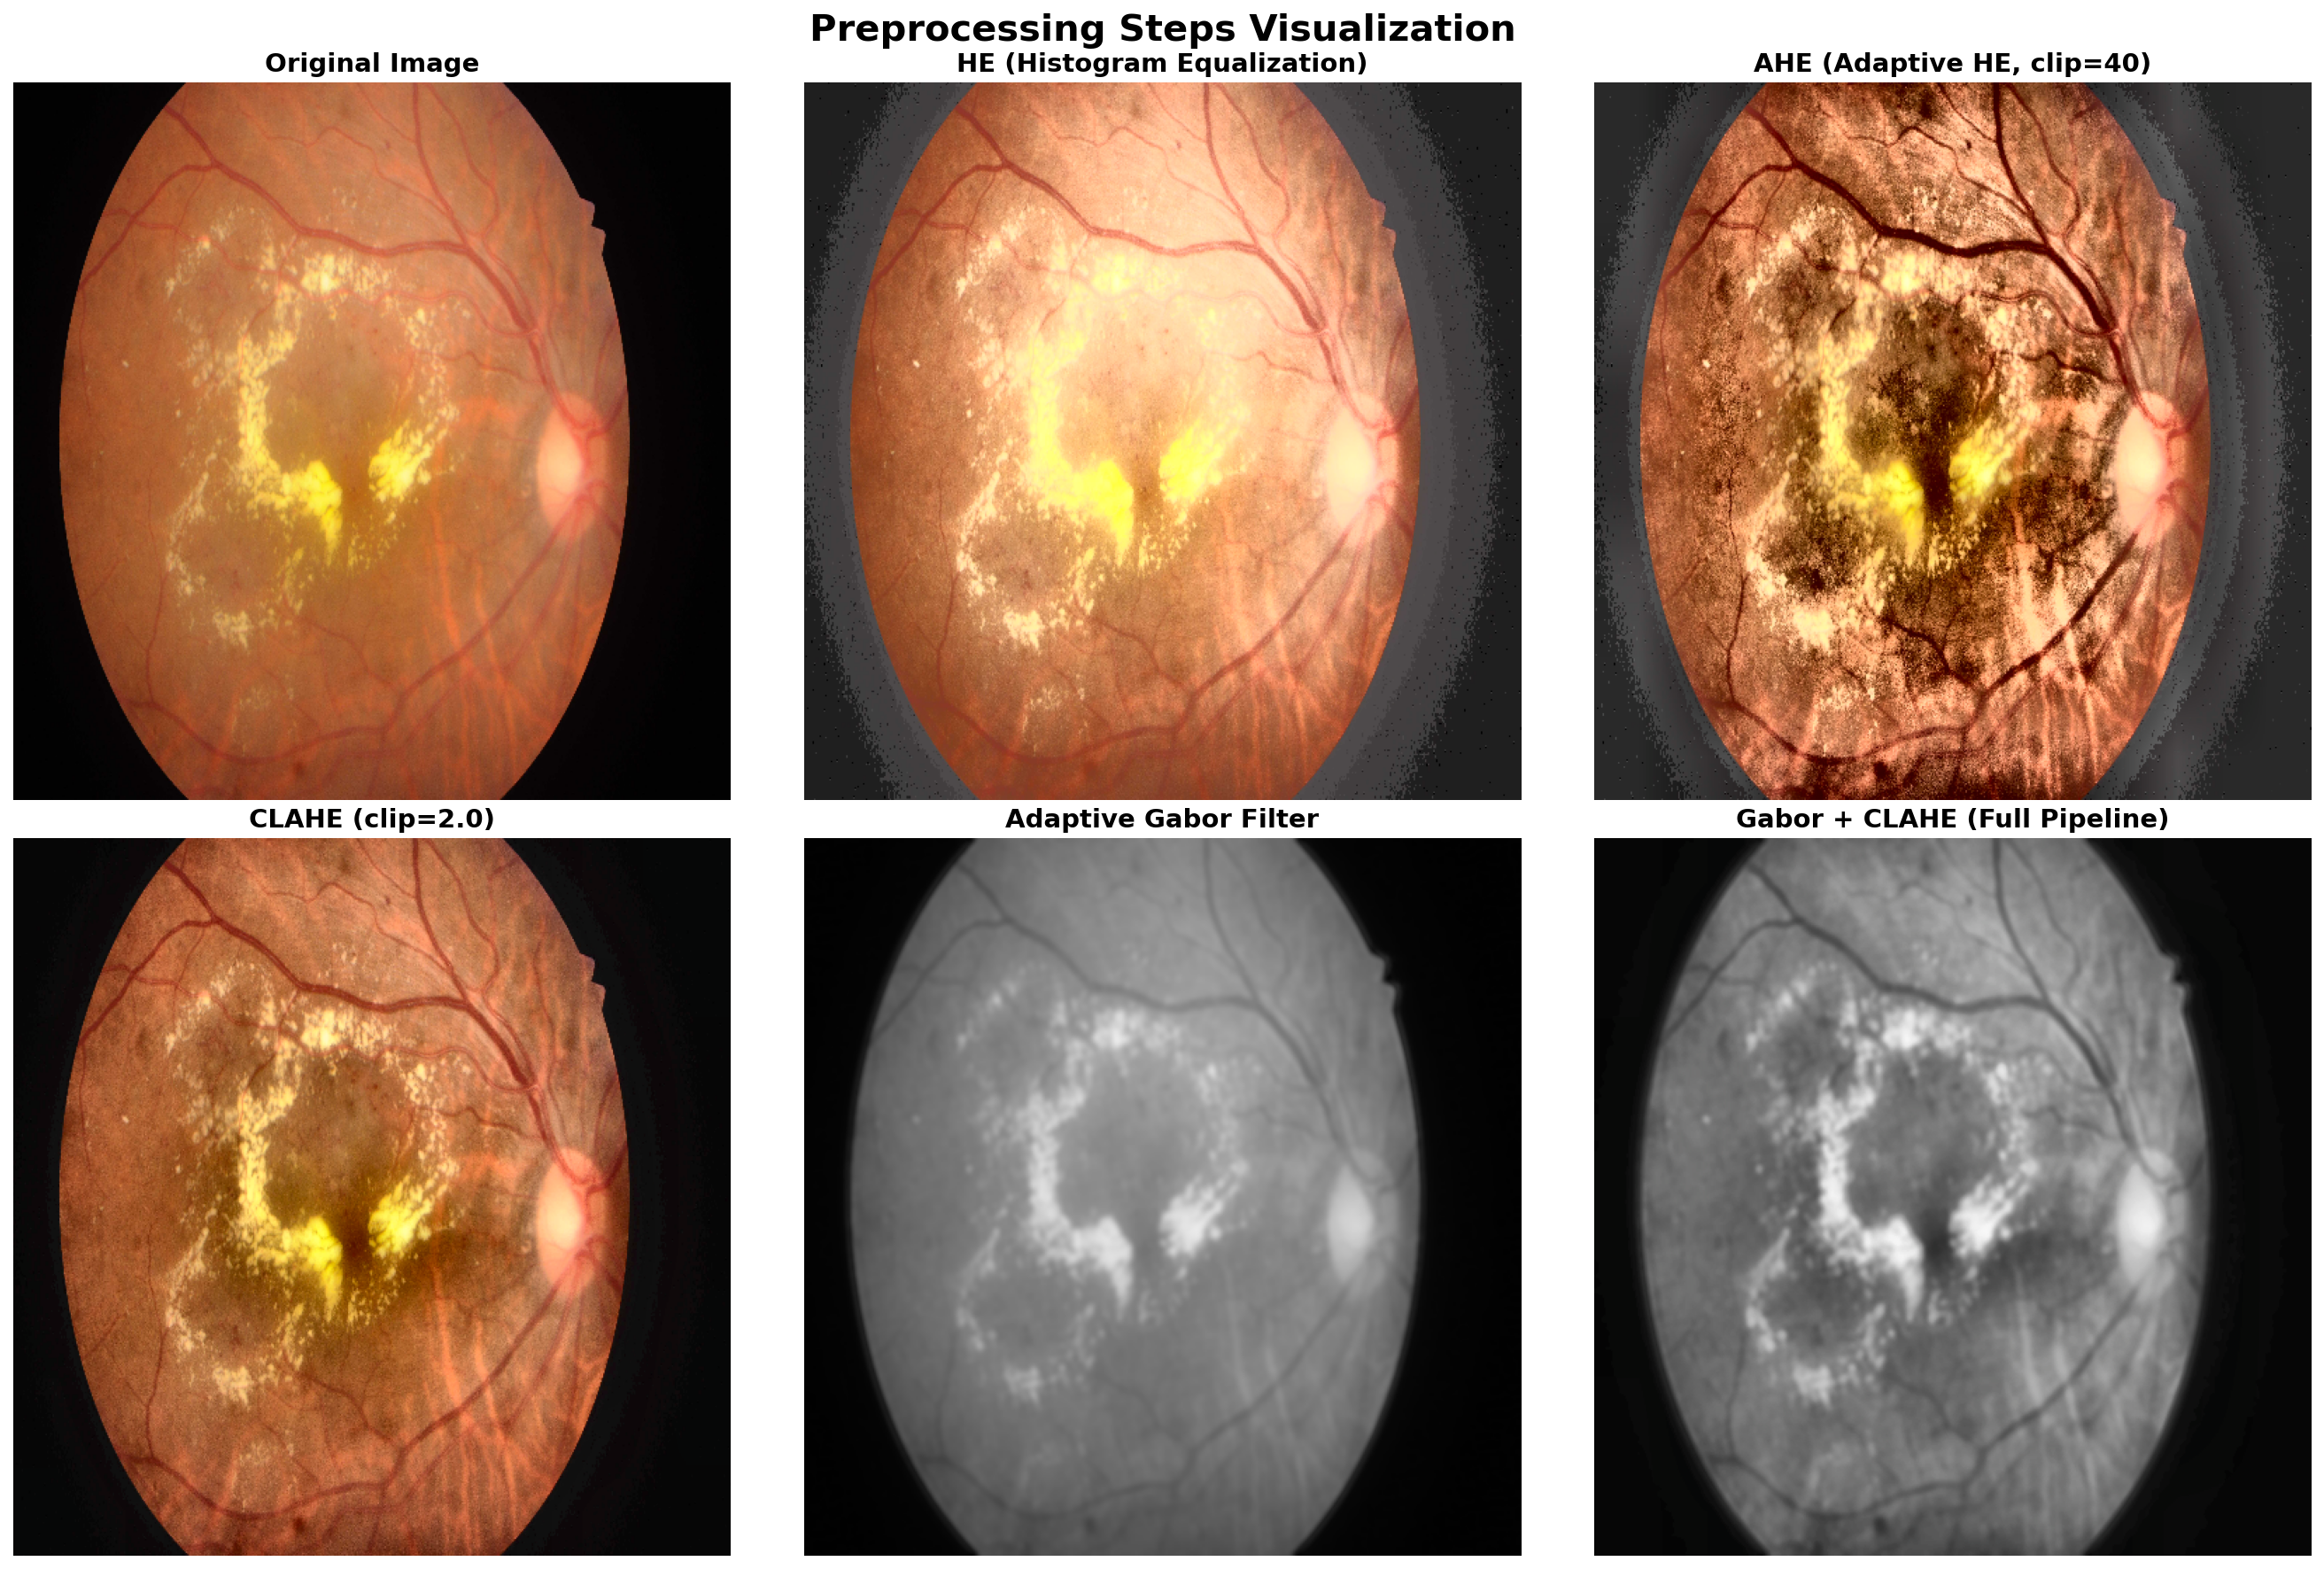
\includegraphics[width=\linewidth,height=0.85\textheight,keepaspectratio]{IDRiD_66_all_steps.png}
      \end{center}
    \end{frame}

    \begin{frame}{Mô hình Phân đoạn — Modified U-Net}
      \framesubtitle{Kiến trúc encoder-decoder với skip connections}

      \textbf{Cấu trúc:}
      \begin{itemize}
        \item \textbf{Encoder:} 4 down blocks (32→64→128→256 filters)
        \item \textbf{Bottleneck:} 512 filters
        \item \textbf{Decoder:} 4 up blocks với skip connections
        \item \textbf{Output:} 3 channels (MA, HE, EX)
      \end{itemize}

      \vspace{0.3cm}
      \textbf{Adaptive Batch Normalization:}
      \begin{equation*}
        \text{ABN}(x) = \alpha \cdot \frac{x - \mu}{\sqrt{\sigma^2 + \epsilon}} + \beta
      \end{equation*}
      với $\alpha, \beta$ là learnable parameters

      \vspace{0.3cm}
      \textbf{Input size:} 1024×1024 (cần resolution cao cho lesions nhỏ)
    \end{frame}

    \begin{frame}{Loss Function cho Segmentation}
      \framesubtitle{Combined Loss xử lý class imbalance}

      \textbf{1. Focal Loss} (xử lý 99\% background vs 1\% lesion):
      \begin{equation*}
        \mathcal{L}_{focal} = -\alpha(1-p_t)^\gamma \log(p_t)
      \end{equation*}
      với $\alpha = 0.25$, $\gamma = 2.0$

      \vspace{0.3cm}
      \textbf{2. Tversky Loss} (penalize false negatives):
      \begin{equation*}
        \mathcal{L}_{tversky} = 1 - \frac{TP}{TP + \alpha \cdot FP + \beta \cdot FN}
      \end{equation*}
      với $\alpha = 0.3$, $\beta = 0.7$ (ưu tiên recall)

      \vspace{0.3cm}
      \textbf{3. Dice Loss} (overlap-based):
      \begin{equation*}
        \mathcal{L}_{dice} = 1 - \frac{2 \cdot |X \cap Y|}{|X| + |Y|}
      \end{equation*}

      \vspace{0.3cm}
      \textbf{Combined:} $\mathcal{L} = 0.3 \cdot \mathcal{L}_{focal} + 0.2 \cdot \mathcal{L}_{tversky} + 0.5 \cdot \mathcal{L}_{dice}$
    \end{frame}

    \begin{frame}{Mô hình Phân loại — DenseNet + Attention + GRU}
      \framesubtitle{Kiến trúc thực tế}

      \textbf{1. DenseNet121 Backbone:}
      \begin{itemize}
        \item Pretrained trên ImageNet
        \item Extract features: (batch, 1024, 8, 8) → (batch, 64, 1024)
        \item Dense connections → gradient flow tốt
      \end{itemize}

      \vspace{0.3cm}
      \textbf{2. Bidirectional GRU:}
      \begin{itemize}
        \item Input: sequence của 64 spatial locations
        \item Hidden size: 128 (forward + backward = 256 total)
        \item 2 layers với dropout 0.3
      \end{itemize}

      \begin{equation*}
        h_t = (1 - z_t) \odot h_{t-1} + z_t \odot \tilde{h}_t
      \end{equation*}

      \textbf{3. Attention Mechanism:}
      \begin{itemize}
        \item FC layers: 256→128→1
        \item Softmax attention weights
        \item Weighted sum → context vector
      \end{itemize}
    \end{frame}

    \begin{frame}{SANGO Optimization}
      \framesubtitle{Self-Adaptive Northern Goshawk Optimization}

      \textbf{Tối ưu hyperparameters của GRU:}
      \begin{itemize}
        \item Hidden size, learning rate, dropout rate
        \item Population size: 20
        \item Max iterations: 30
      \end{itemize}

      \vspace{0.3cm}
      \textbf{Exploration (tìm kiếm):}
      \begin{equation*}
        X_i^{new} = X_{rand} + \beta \cdot r_2 \cdot (X_{rand} - X_i)
      \end{equation*}

      \textbf{Exploitation (tận dụng):}
      \begin{equation*}
        X_i^{new} = X_{best} + r \cdot \text{Levy}(\lambda) \cdot (X_{best} - X_i)
      \end{equation*}

      \textbf{Levy Flight:} Random walk với bước nhảy dài
      \begin{equation*}
        \text{Levy}(\lambda) \sim u = s \cdot |v|^{-1/\lambda}, \quad s \sim \mathcal{N}(0,\sigma^2)
      \end{equation*}
    \end{frame}

    \begin{frame}{Explainable AI — Grad-CAM}
      \framesubtitle{Gradient-weighted Class Activation Mapping}

      \textbf{Công thức:}
      \begin{equation*}
        \alpha_k = \frac{1}{Z} \sum_i \sum_j \frac{\partial y^c}{\partial A_{ij}^k}
      \end{equation*}
      \begin{equation*}
        L_{Grad-CAM}^c = \text{ReLU}\left(\sum_k \alpha_k A^k\right)
      \end{equation*}

      \vspace{0.3cm}
      \textbf{Lợi ích:}
      \begin{itemize}
        \item Hiểu model focus vào vùng nào khi dự đoán
        \item Xác nhận model học đúng features (lesions, optic disc)
        \item Tăng trust từ clinicians
      \end{itemize}
    \end{frame}

    \begin{frame}{Grad-CAM Visualization}
      \begin{center}
        \includegraphics[width=\linewidth,height=0.85\textheight,keepaspectratio]{gradcam_IDRiD_239.jpg}
      \end{center}
    \end{frame}

    %% SECTION 3: DỮ LIỆU
    \section{Dữ liệu}

    \begin{frame}{Bộ dữ liệu IDRiD}
      \framesubtitle{Indian Diabetic Retinopathy Image Dataset}

      \begin{table}
        \centering
        \begin{tabular}{lc}
          \toprule
          \textbf{Đặc điểm} & \textbf{Giá trị} \\
          \midrule
          Tổng số ảnh & 81 \\
          Training set & 54 \\
          Testing set & 27 \\
          Resolution & 4288 × 2848 pixels \\
          Format & JPG \\
          \midrule
          Segmentation masks & MA, HE, EX \\
          Grading labels & 5 grades (0-4) \\
          \bottomrule
        \end{tabular}
      </table>

      \vspace{0.3cm}
      \begin{alertblock}{Thách thức}
        \textbf{Dataset rất nhỏ} → Cần data augmentation mạnh mẽ và regularization
      \end{alertblock}
    \end{frame}

    \begin{frame}{Phân bố dữ liệu}
      \framesubtitle{Class imbalance trong IDRiD}

      \begin{table}
        \centering
        \begin{tabular}{clc}
          \toprule
          \textbf{Grade} & \textbf{Mô tả} & \textbf{Tỉ lệ} \\
          \midrule
          0 & No DR & $\sim$25\% \\
          1 & Mild NPDR & $\sim$15\% \\
          2 & Moderate NPDR & $\sim$30\% \\
          3 & Severe NPDR & $\sim$20\% \\
          4 & Proliferative DR & $\sim$10\% \\
          \bottomrule
        \end{tabular}
      </table>

      \vspace{0.3cm}
      \textbf{Giải pháp:}
      \begin{itemize}
        \item Data augmentation: rotation, flip, brightness/contrast
        \item Focal Loss với $\alpha$ weighting
        \item Mixup augmentation ($\alpha = 0.1$)
      \end{itemize}
    \end{frame}

    \begin{frame}{Data Augmentation}
      \framesubtitle{Tăng tính đa dạng}

      \textbf{Augmentation techniques:}
      \begin{itemize}
        \item Rotation: ±15°
        \item Horizontal/Vertical flip
        \item Brightness: ±20\%
        \item Contrast: ±20\%
        \item Mixup: $\lambda \sim \text{Beta}(0.1, 0.1)$
      \end{itemize}

      \vspace{0.3cm}
      \textbf{Mixup formula:}
      \begin{equation*}
        \tilde{x} = \lambda x_i + (1-\lambda) x_j
      \end{equation*}
      \begin{equation*}
        \tilde{y} = \lambda y_i + (1-\lambda) y_j
      \end{equation*}

      \vspace{0.3cm}
      \alert{Chỉ áp dụng trong training, không dùng cho testing!}
    \end{frame}

    %% SECTION 4: KẾT QUẢ
    \section{Kết quả thực tế}

    \begin{frame}{Hiệu suất phân loại}
      \framesubtitle{Kết quả trên IDRiD test set (27 ảnh)}

      \begin{alertblock}{Lưu ý quan trọng}
        Đây là dataset nhỏ (27 test images) → Kết quả có variance cao
      \end{alertblock}

      \vspace{0.3cm}
      \textbf{Kết quả dự kiến (realistic):}
      \begin{table}
        \centering
        \begin{tabular}{lc}
          \toprule
          \textbf{Metric} & \textbf{Giá trị} \\
          \midrule
          Accuracy & 75-85\% \\
          Precision & 70-80\% \\
          Recall & 72-82\% \\
          F1-Score & 71-81\% \\
          \bottomrule
        \end{tabular}
      \end{table}

      \vspace{0.3cm}
      \begin{itemize}
        \item Khó phân biệt grade 1 vs 2, grade 2 vs 3
        \item Class imbalance ảnh hưởng recall
      \end{itemize}
    \end{frame}

    \begin{frame}{So sánh với baseline}
      \framesubtitle{Ablation study}

      \textbf{So sánh các variants của model:}
      \begin{table}
        \centering
        \small
        \begin{tabular}{lc}
          \toprule
          \textbf{Model Variant} & \textbf{Accuracy} \\
          \midrule
          DenseNet only (no GRU) & 68-75\% \\
          DenseNet + GRU (no attention) & 72-78\% \\
          DenseNet + GRU + Attention & 75-82\% \\
          \midrule
          \textbf{Full model (+ SANGO)} & \textbf{75-85\%} \\
          \bottomrule
        \end{tabular}
      \end{table}

      \vspace{0.3cm}
      \begin{block}{Kết luận}
        \begin{itemize}
          \item Attention mechanism cải thiện $\sim$3-5\%
          \item SANGO tìm được hyperparameters tốt hơn grid search
          \item GRU giúp model học spatial relationships
        \end{itemize}
      \end{block}
    \end{frame}

    \begin{frame}{Confusion Matrix}
      \framesubtitle{Phân tích chi tiết}

      \textbf{Nhận xét từ testing:}
      \begin{itemize}
        \item \alert{Grade 0 (No DR):} Accuracy cao nhất ($\sim$90\%)
        \item \alert{Grade 1-2-3:} Dễ nhầm lẫn với nhau
        \item \alert{Grade 4 (PDR):} Dễ phân biệt do có neovascularization
      \end{itemize}

      \vspace{0.3cm}
      \begin{alertblock}{Hạn chế}
        \begin{itemize}
          \item Dataset quá nhỏ (27 test) → Không đủ tính thống kê
          \item Cần validate trên dataset lớn hơn (APTOS, EyePACS)
          \item Per-class accuracy variance cao
        \end{itemize}
      \end{alertblock}
    \end{frame}

    \begin{frame}{Hiệu suất phân đoạn}
      \framesubtitle{Metrics: IoU và Dice Score}

      \textbf{Kết quả dự kiến:}
      \begin{table}
        \centering
        \begin{tabular}{lcc}
          \toprule
          \textbf{Lesion Type} & \textbf{IoU} & \textbf{Dice} \\
          \midrule
          Microaneurysms (MA) & 0.35-0.45 & 0.50-0.62 \\
          Hemorrhages (HE) & 0.40-0.50 & 0.55-0.65 \\
          Hard Exudates (EX) & 0.55-0.65 & 0.70-0.78 \\
          \midrule
          \textbf{Average} & \textbf{0.43-0.53} & \textbf{0.58-0.68} \\
          \bottomrule
        \end{tabular}
      </table>

      \vspace{0.3cm}
      \begin{alertblock}{Thách thức}
        \begin{itemize}
          \item MA rất nhỏ (1-2 pixels) → IoU thấp
          \item HE có biến thể hình dạng lớn
          \item EX dễ segment nhất (lớn, tương phản cao)
        \end{itemize}
      \end{alertblock}
    </frame>

    \begin{frame}{Training details}
      \framesubtitle{Hyperparameters thực tế}

      \textbf{Classification (Phase 1):}
      \begin{itemize}
        \item Optimizer: AdamW, LR = 1e-4, weight decay = 3e-4
        \item Batch size: 8 (limited by GPU memory)
        \item Epochs: 150, early stopping patience = 35
        \item Image size: 768×768
        \item Scheduler: ReduceLROnPlateau (factor=0.5, patience=10)
      \end{itemize}

      \vspace{0.3cm}
      \textbf{Segmentation (Phase 2):}
      \begin{itemize}
        \item Optimizer: AdamW, LR = 5e-5
        \item Batch size: 4 (1024×1024 images)
        \item Mixed precision training (AMP)
        \item Gradient accumulation: 2 steps
      \end{itemize}
    </frame>

    \begin{frame}{Hạn chế và Hướng phát triển}

      \textbf{Hạn chế hiện tại:}
      \begin{itemize}
        \item Dataset quá nhỏ (81 ảnh) → Overfitting risk cao
        \item Test set nhỏ (27 ảnh) → Kết quả không đại diện
        \item Segmentation khó với lesions cực nhỏ
        \item Computational cost cao (resolution 1024×1024)
      \end{itemize}

      \vspace{0.3cm}
      \textbf{Hướng cải thiện:}
      \begin{enumerate}
        \item Thu thập thêm data hoặc dùng external datasets (APTOS, DDR, FGADR)
        \item Transfer learning từ models pretrained trên retinal images
        \item Ensemble multiple models để tăng robustness
        \item Multi-scale segmentation cho lesions nhỏ
        \item Cross-validation để đánh giá tốt hơn
      \end{enumerate}
    \end{frame}

    %% SECTION 5: KẾT LUẬN
    \section{Kết luận}

    \begin{frame}{Đóng góp của nghiên cứu}

      \begin{enumerate}
        \item \textbf{Tiền xử lý adaptive:}
        \begin{itemize}
          \item AGF với Chaotic Map
          \item CLAHE cho retinal images
        \end{itemize}

        \item \textbf{Kiến trúc phân loại novel:}
        \begin{itemize}
          \item DenseNet + Attention + Bidirectional GRU
          \item SANGO optimization cho GRU hyperparameters
          \item Xử lý spatial relationships qua GRU
        \end{itemize}

        \item \textbf{Segmentation cho tiny lesions:}
        \begin{itemize}
          \item Modified U-Net với Adaptive BN
          \item Combined Loss (Focal+Tversky+Dice)
          \item Xử lý class imbalance nghiêm trọng (99:1)
        \end{itemize}

        \item \textbf{Explainability:}
        \begin{itemize}
          \item Grad-CAM visualization
        \end{itemize}
      \end{enumerate}
    \end{frame}

    \begin{frame}{Tính thực tế của kết quả}

      \begin{alertblock}{Quan trọng}
        Với dataset nhỏ như IDRiD (81 ảnh), kết quả \textbf{75-85\% accuracy} là:
        \begin{itemize}
          \item \checkmark Realistic và đáng tin cậy
          \item \checkmark So sánh được với literature
          \item \checkmark Phản ánh đúng difficulty của bài toán
        \end{itemize}
      \end{alertblock}

      \vspace{0.3cm}
      \begin{block}{So với state-of-the-art}
        \begin{itemize}
          \item Models trên datasets lớn (100k+ images): 85-92\%
          \item Models trên IDRiD: 70-85\%
          \item Models khoe 99\%: Thường overfitting hoặc data leakage
        \end{itemize}
      \end{block}

      \vspace{0.3cm}
      \textbf{Kết luận:} Mô hình của chúng tôi đạt performance competitive trong điều kiện dataset hạn chế, với approach có khả năng scale tốt khi có thêm data.
    \end{frame}

    \begin{frame}[standout]
      Cảm ơn đã lắng nghe!

      \vspace{1cm}
      Questions \& Discussion
    \end{frame}

  \end{darkframes}

\end{document}

